\chapter{An SVM for structured errors} \label{chap:dsvm}
\begin{sloppypar}
\lettrine{N}{on-stationary} feature distributions violate the basic assumption
made by most \ac{ML} methods that the data is \ac{IID}. In
Chapter~\ref{chap:sob}, we demonstrated for the first time that cross-subject
\ac{EEG} classification is possible by making the training set's and test set's
distribution similar with a normalization procedure. But this normalization
procedure does not result in a performance gain with \acf{SD} application (i.e.
the usual scenario where a calibration session is used before application).
%
This is consistent with prior work on non-stationary signals in \acp{BCI} that
attempts to reduce feature variability over time \cite{hill2006tdd,
tomioka2006asf, blankertz2007ics, bunau2009ssa, meinecke2009lis,
reuderink2010sss} or alternatively to adapt the classifier's parameters to the
changing distribution \cite{shenoy2006tac, vidaurre2007sol}, where at best
modest improvements are reported.
\end{sloppypar}

It is unclear to what degree variability in the feature distributions
influences the \ac{SD} \ac{BCI}, since the variable features might be
irrelevant to the specific classification problem. The \ac{SSA} method
\cite{bunau2009ssa, meinecke2009lis} hinges on this assumption. But even if
this assumption holds, attempting to remove the irrelevant variability could
introduce residual noise. As a consequence the performance could suffer, while
a robust classifier might have been able to learn these variations in the data
in the first place. This may be the reason why most of the aforementioned
studies have been demonstrated on datasets that were artificially augmented
with strong non-stationary distributions, or had to include additional data or
labels to learn from.

All these proposed methods focus on assuring that the features are identically
distributed during training and testing. Still, being identically distributed
does not imply that the samples are independent of each other.
%
The dependence of trials over time, which can be caused for example by inertia
of neural processes or by filtering artifacts (or even the \ac{SOB} procedure), can result in prediction errors
that are dependent in time. 
%
If the classifier observes a series of dependent errors that are caused by a
single (hidden) event, and assumes that these errors are unrelated, this can
severely bias the classifier and lead to overfitting.
%
Incorporating a priori known dependencies in the model thus enables the
classifier to reduce the penalty for related errors (e.g. caused by a period of
distraction of the user) and to focus on structural errors present in the data.
 
In this Chapter, we focus on the violation of the independence aspect of the
\ac{IID} assumption. Instead of attempting to remove dependencies in the
feature space as done in previous work, we modeled the dependencies in the
objective function of the classifier. Specifically, we present a generalization
of the \ac{SVM} that uses latent slack variables to model the structure
of misclassified training instances. By penalizing these latent slack
variables, the \ac{dSVM} was able to diminish the influence of related errors
and to reduce overfitting. The \ac{dSVM} was evaluated on real \ac{BCI}
datasets, and showed an improvement in performance.

\section{Previous work}
\section{Previous work}
The influence of frustration associated with \ac{LOC} on a
\ac{BCI} is of great interest since it might cause the previously described
feedback loop. This influence  was previously investigated in
\cite{jatzev2008ecn, zander2009usi}. In this study, users were instructed to
use real movement with their left or right hand to rotate respectively L or
R-shaped objects to a target position in order to study the effect of \acl{LOC}
on the \ac{BCI} performance.
%
The color of the letter indicated the angle of rotation, and the user could
press a key to rotate the object in the direction indicated by the shape of the
object every second.
%
After performing a calibration block with cued left/right hand movement and two
practise blocks with this so-called RLR paradigm, a \ac{LOC} was simulated in
the third block by occasionally using a wrong angle of rotation in the
application. Both an \ac{ERD} and an \ac{ERP} based classifier were trained on
the first block, and applied to the other blocks in an off-line analysis.  A
significant difference between the training block and the \ac{LOC} block was
found for the distribution of \ac{ERD} based features, but for \ac{ERP}
features no such difference was found. This seems to indicate that there is
variability in \ac{ERD} features related to \acl{LOC}. 

However, the study described in \cite{jatzev2008ecn, zander2009usi} is lacking
on a few aspects. Most notable is the limitation that changes in \ac{BCI}
performance due to the induction of \ac{LOC}, the progression of time,
differences in stimulation and user behaviour cannot be distinguished.
%
We were interested in the influence of \ac{LOC} on the \ac{BCI} performance
independent of these other factors. Therefore we used 1) an interleaved block
design to control for effects that manifest spontaneously over time, such as
increasing fatigue, changing temperature, drying gel on the electrodes etc., 2)
we used the same environment for training and evaluating the \ac{BCI}
classifiers to minimize environmental differences not related to \ac{LOC}, 3)
we used self-reported emotional ratings to validate the effect of \acl{LOC} on
the mental state and 4) we tested and corrected for confounding behavioural
changes, such as changes in the force, speed or order of the finger movements,
and eye movements. 


\section{The dependent-samples SVM}
\begin{sloppypar}
Given training examples $\{\vec{x}_i\}$ and corresponding labels $\vec{y}_i \in
\{-1, 1\}$, the \ac{dSVM} can be formulated as the following constrained,
convex optimization problem:
\begin{align}
  \arg\min_{\vec{w},b,\xi} \quad
  & \frac{1}{2}\norm{\vec{w}}^2 
  + c \sum_i \vec{\xi}_i
\\
  \text{s.t.} \quad 
  & y_i \left(\vec{w}^T \phi(\vec{x}_i) + b\right) + D \vec{\xi}_i \ge 1
\\
  & \vec{\xi}_i \ge 0,
\end{align}
%
where $\vec{w}$ is the classifier's weight vector and $b$ is the bias term.
The function $\phi(\cdot)$ maps examples from input space to a feature space.
The $c$ parameter determines the cost of penetrating the \ac{SVM}'s
margin (margin errors); $\vec{\xi}_i$ is a positive, latent slack-variable that
accommodates for these margin errors, and is related to a specific example $i$
through $(D\vec{\xi})_i$. 
%
When $D$ is the identity matrix $I$, each slack variable $\vec{\xi}_i$ is
linked to a single instance $i$ of the training set, and the \ac{dSVM}
degenerates to the traditional soft-margin \ac{SVM} \cite{cortes1995svn}. The
columns $D_{i,\cdot}$ contain the non-negative dispersion function for a
specific latent error $\vec{\xi}_i$ that needs to be specified a priori.
\end{sloppypar}

%
For ease of notation, we write this in matrix form 
with $Y_{i,i} = \vec{y}_i$ and $X_{\cdot,i} = \phi(x_i)$:
\begin{align}
  \arg\min_{\vec{w}, b, \vec{\xi}} \quad
  & \frac{1}{2}\norm{\vec{w}}^2
  + c\vec{\xi}^T\vec{1}
\\ \label{eq:dsvm_margin_error_const}
  \text{s.t.} \quad &
  Y \left(\vec{w}^T X + b\right)^T + D \vec{\xi} - 1 \succeq 0 
\\&
  \vec{\xi} \succeq 0.
\end{align}
%
With the Lagrange multipliers $\vec{\alpha}$ and $\vec{\gamma}$, the
constraints can be put in the primal objective function $\mathcal{L}_p$ that
needs to be minimized for $\vec{w}$ and $b$, and maximized for the
dual variables $\vec{\alpha}$ and $\vec{\gamma}$:
\begin{align}
  \mathcal{L}_p(\vec{w}, b, \vec{\xi}, \vec{\alpha}, \vec{\gamma})= & 
  \frac{1}{2} \vec{w}^T \vec{w}
  + c\vec{\xi}^T\vec{1}
  - \vec{\alpha}^T \left(
    Y X^T \vec{w} + b \vec{y}  + D \vec{\xi} - \vec{1}
    \right)
  - \vec{\gamma}^T \vec{\xi}
\\
  \text{s.t.} \quad &
  \vec{\alpha} \succeq 0 \quad \text{and} \quad \vec{\gamma} \succeq 0,
  \label{eq:dsvm_slack_const}
\end{align}
%
Setting the derivative of the primal variables $\vec{w}$, $b$ and $\vec{\xi}$ to zero yields their minimum,
\begin{align}
  \frac{\delta}{\delta \vec{w}} \mathcal{L}_p &= 
  \vec{w}^T - \vec{\alpha}^T Y X^X = 0
  &&\Rightarrow \vec{w} = X Y \vec{\alpha}
  \label{eq:dsvm_w_prime}
\\
  \frac{\delta}{\delta b} \mathcal{L}_p &= 
  -\vec{\alpha}^T \vec{y} = 0
  &&\Rightarrow \vec{\alpha}^T \vec{y} = 0
  \label{eq:dsvm_b_prime}
\\
  \frac{\delta}{\delta \vec{\xi}} \mathcal{L}_p &= 
  c\vec{1}^T - \vec{\alpha}^T D - \vec{\gamma}^T = 0
  &&\Rightarrow c\vec{1}^T = \vec{\alpha}^T D + \vec{\gamma}^T,
  \label{eq:dsvm_xi_prime}
\end{align}
%
that result in the dual $\mathcal{L}_d$ after substitution:
\begin{align} % substitute w
%  \mathcal{L}_d & =
%  \frac{1}{2} 
%    \vec{\alpha}^T Y X^T X Y \vec{\alpha}
%  + c\vec{\xi}^T\vec{1}
%  - \vec{\alpha}^T \left(
%    Y X^T X Y \vec{\alpha} 
%      + D \vec{\xi} 
%      - \vec{1}
%    \right)
%  - \vec{\gamma}^T \vec{\xi}
%\\ & =
%  \vec{\alpha}^T \vec{1}
%  - \frac{1}{2} \vec{\alpha}^T Y K Y \vec{\alpha}
%  + c \vec{1}^T\vec{\xi}
%  - \vec{\alpha}^T D \vec{\xi} 
%  - \vec{\gamma}^T \vec{\xi}
%\\ & =
%  \vec{\alpha}^T \vec{1}
%  - \frac{1}{2} \vec{\alpha}^T Y K Y \vec{\alpha}
%  + \left(
%    c \vec{1}^T
%    - \vec{\alpha}^T D
%    - \vec{\gamma}^T
%    \right) \vec{\xi}
%\\
  \mathcal{L}_d (\vec{\alpha}) & =
  \vec{\alpha}^T \vec{1}
  - \frac{1}{2} \vec{\alpha}^T Y K Y \vec{\alpha},
\end{align}
%
where the kernel matrix $K_{i,j}=\phi(\vec{x_i})^T \phi(\vec{x_j})$.
The dual $\mathcal{L}_d$ needs to be maximized with respect to the dual
variables $\vec{\alpha}$, subject to the \ac{KKT} conditions
\eqref{eq:dsvm_b_prime}, \eqref{eq:dsvm_xi_prime} and
\eqref{eq:dsvm_slack_const}:
%
\begin{align}
  \arg\max_{\vec{\alpha}} \quad \mathcal{L}_d = & 
  \vec{\alpha}^T \vec{1} - \frac{1}{2} \vec{\alpha}^T Y K Y \vec{\alpha}
  \label{eq:dsvm_dual}
\\
  \text{s.t.} \quad &
  0 \preceq \vec{\alpha}^T D \preceq c, \quad \vec{\alpha}^T \vec{y} = 0.
  \label{eq:dsvm_dual_const}
\end{align}
%
The only difference of this dual with the soft-margin \ac{SVM}'s dual is the
appearance of the dispersion matrix $D$ in the constraint
\eqref{eq:dsvm_dual_const}; with $D=I$ the dual degenerates to the soft-margin \ac{SVM}'s
dual. 
%
The \ac{dSVM}'s dual \eqref{eq:dsvm_dual} and constraints
\eqref{eq:dsvm_dual_const} form a \ac{QP} problem, and an optimal
$\vec{\alpha}$ can be found with a standard \ac{QP} solver. With $\vec{\alpha}$
found, $\vec{w}$ is defined through \eqref{eq:dsvm_w_prime}. 

The bias $b$ is usually calculated from support vectors on the
boundary of the margin using \eqref{eq:dsvm_margin_error_const} in the
traditional soft-margin \ac{SVM} formulation, i.e. from the $x_i$ where
$\vec{\alpha}_i > 0$ and $(I\vec{\xi})_i = 0$. 
%For these unconstrained support vectors, the term $YD \vec{\xi}$ in
%
%\begin{align}
%  Y \left(\vec{w}^T X + b\right)^T + D \vec{\xi} - 1 &\succeq 0 
%\\
%  Y \left(\vec{w}^T X + \vec{b}^T\right)^T + D \vec{\xi} - 1 &\succeq 0 
%\\
%  Y \left(X^T\vec{w} + \vec{b}\right) + D \vec{\xi} - 1 &\succeq 0 
%\\
%  Y X^T\vec{w} + Y\vec{b} + D \vec{\xi} - 1 &\succeq 0 
%\\
%  Y\vec{b} &\succeq 1 - D \vec{\xi} - Y X^T\vec{w}
%\\
%  \vec{b} &\succeq Y^{-1}\vec{1} - Y^{-1}D \vec{\xi} - Y^{-1}Y X^T \vec{w}
%\\
%  \vec{b} &\succeq Y\vec{1} - YD \vec{\xi} - K Y \vec{\alpha}
%\\
%  \label{eq:dsvm_bias}
%  \vec{b} &\succeq \vec{y} - K Y \vec{\alpha} - YD \vec{\xi}
%\end{align}
%vanishes, and $b$ can be calculated from the known kernel, labels and
%$\vec{\alpha}$.
%
%It is possible however, that there are no unconstrained support vectors, and
%$b$ is optimal for an interval. 
With the \ac{dSVM}, this definition of unconstrained support vectors is
troublesome, since the latent slack variables are associated with multiple
(possibly all) support vectors through $D$. Therefore, we have chosen to use an
implicit, regularized bias instead, which can be implemented by either adding a
constant feature, or by using an inhomogeneous kernel. To remove the bias term,
the constraint \eqref{eq:dsvm_b_prime} has to be removed, resulting in
%
\begin{align}
  \arg\min_{\vec{\alpha}} \quad \mathcal{L}_d = & 
  \frac{1}{2} \vec{\alpha}^T Y K Y \vec{\alpha}
  - \vec{1}^T\vec{\alpha}
\\
  \text{s.t.} \quad &
  0 \preceq \vec{\alpha}^T D \preceq c,
\end{align}
which is still a standard \ac{QP} problem.

\begin{sloppypar}
Classification with the \ac{dSVM} is done as with the \ac{SVM}, using
\eqref{eq:dsvm_w_prime} and \eqref{eq:dsvm_margin_error_const}, with $b=0$:
%
\begin{equation}
  f(X_2) = \vec{w}^T X_2 + b = \vec{\alpha}^T Y X^T X_2 = \vec{\alpha}^T Y K_2.
\end{equation}
%
The main difference between the \ac{dSVM} and the traditional soft-margin
\ac{SVM} is that \ac{dSVM} has groups of support vectors that share a ``support
budget'', whereas the former has a budget per support vector. In addition, the
dispersion matrix $D$ has to be specified a priori based on domain knowledge
(e.g. for time series classification with a sliding window, the dependence is
apparent from the feature construction).
%
The dispersion functions (columns of $D$) do not have to be the same function
with an offset. For example, when combining the data of multiple subjects, the
$D$ matrix could model a dependency of all trials (instances) on a subject, and
a dependency on trials of the same subject near in time. This would allow the
\ac{dSVM} to remove subjects that do not display the expected brain signal
altogether from the training set, while still spending modeling power on an as 
diverse set of subjects as possible.
\end{sloppypar}


\section{Validation}
To validate the \ac{dSVM} introduced in the previous section, we constructed an
artificial dataset to demonstrate the \ac{dSVM}'s robustness against dependent
disturbances. After demonstrating the \ac{dSVM} on this artificial dataset, we
will present the evaluation of the \ac{dSVM} on a real \ac{BCI} dataset.

\subsection{Artificial data}
The dataset was constructed by sampling from two Gaussian distributions with
equal covariance but different means. A non-stationary perturbation
in feature space was generated with the Laplace distribution function
\begin{align} \label{eq:laplace_dist}
  f(x \vert \mu, b) = \frac{1}{2b} e^{-\frac{\lvert x - \mu\rvert}{b}},
\end{align}
with $b=9$ and $\mu=60$, where the argument $x$ is the position in the dataset.
This makes the instances non-\ac{IID} (see Figure~\ref{fig:artdata}), with a known dispersion function.

\begin{figure}
  \center
  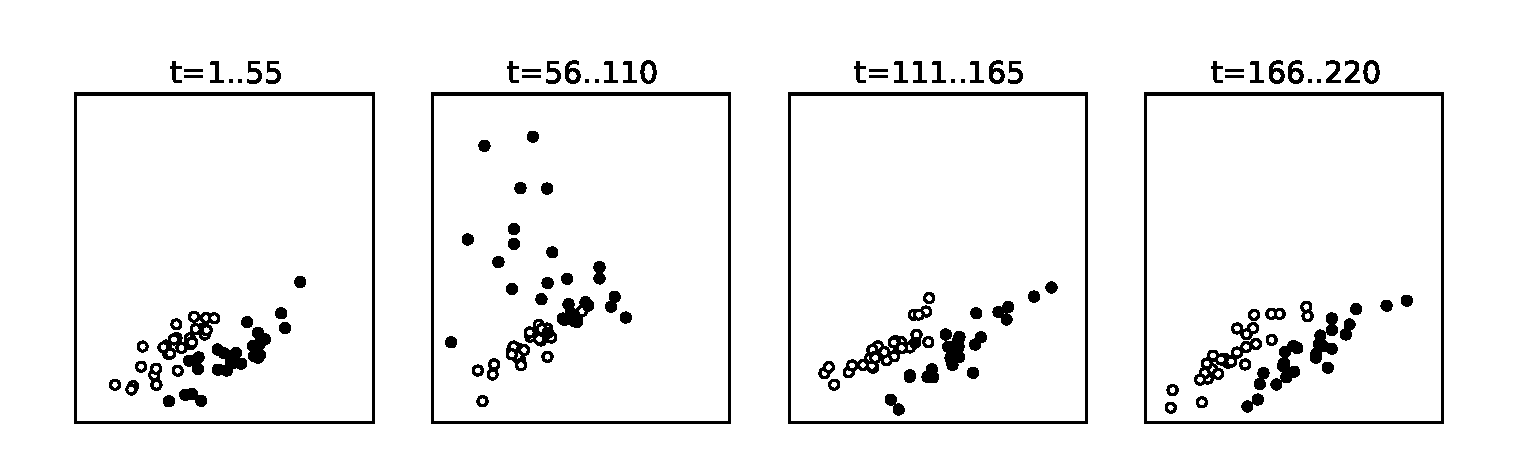
\includegraphics[width=\textwidth]{artdata.pdf}
  \caption{Sequential snapshots of the artificial dataset used to evaluate the
    \protect\ac{dSVM}. The data is sampled form two Gaussian distributions with
    different means but equal covariance. In the second frame, we introduce a
    latent error, that leaks to a range of related of samples.}
  \label{fig:artdata}
\end{figure}

A Laplace distribution was chosen based on its similarity to the empirical
distribution found in a preliminary experiment, in which we modeled the
interdependence of slack variables in the training set of a \ac{BCI}
experiment. As the strongest dependence in this preliminary experiment was
found between slack variables of the same class, the perturbation was limited
to one class only.

\begin{sloppypar}
Both a soft-margin \ac{SVM} and a \ac{dSVM} were trained on this artificially
constructed dataset. Model selection for the cost parameter $c$ was performed
with a line search on cross-validated accuracy with four sequential subsets
corresponding to the frames in Figure~\ref{fig:artdata}. The \ac{dSVM}'s
dispersion matrix $D$ was constructed using \eqref{eq:laplace_dist}:
%
\begin{align} \label{eq:dfunc}
  \tilde{D}_{i,j} &=
    \begin{cases}
      g_i \cdot f(\lvert t_i - t_j \rvert) 
        & \text{if } y_i = y_j,
    \\
      0 & \text{otherwise}
    \end{cases}
\end{align}
where $t_i$ is the time offset of an instance $i$, and $\vec{g}$ chosen such
that the columns of $D$ are normalized to one.
\end{sloppypar}

\begin{figure}
  \center
  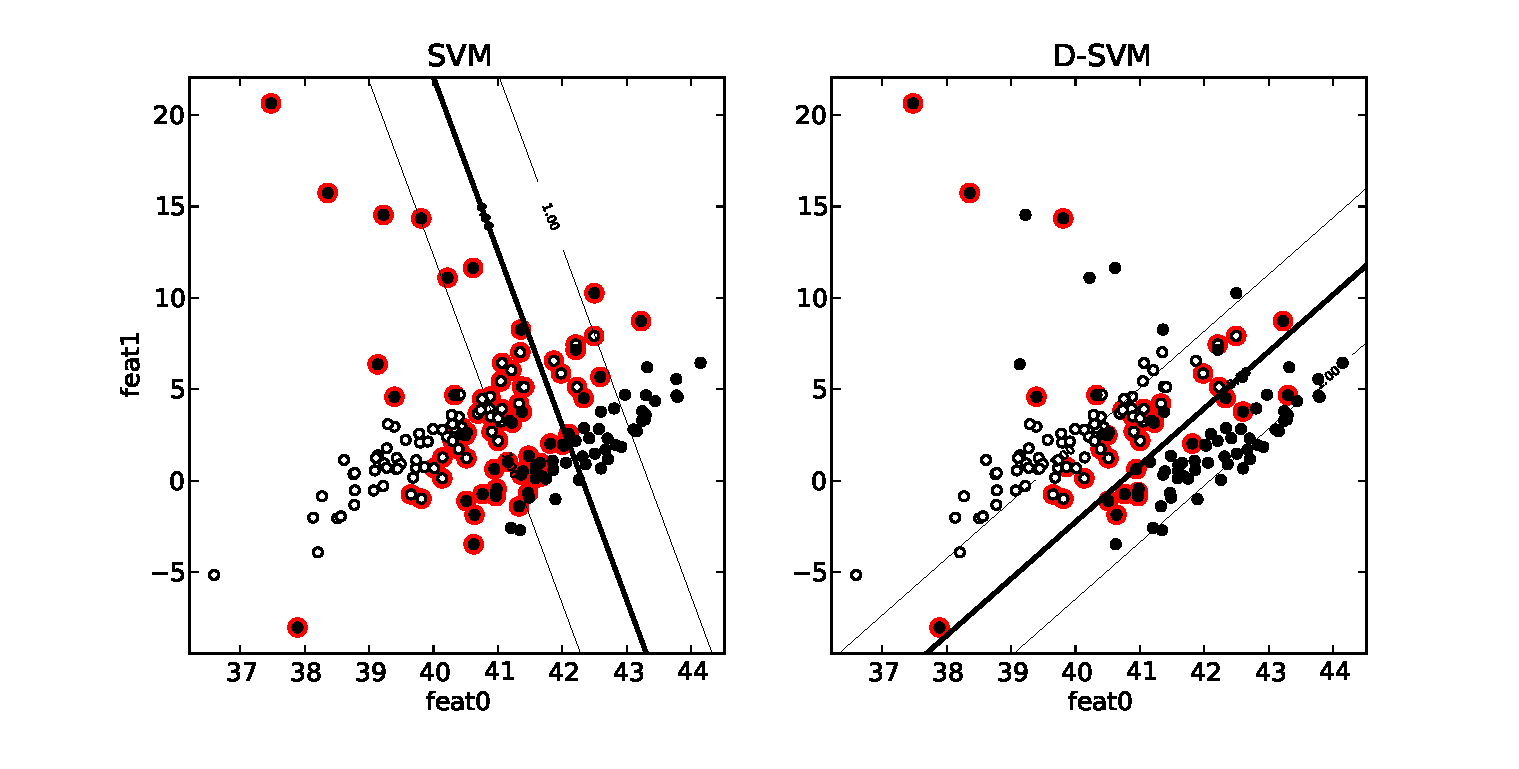
\includegraphics[width=\textwidth]{svm_vs_dsvm.pdf}
  \caption{The hyperplane (thick black line) and margin (between the thin black
    lines) for the standard soft-margin \protect\ac{SVM} (left) and the
    \protect{dSVM} (right). Both classifiers were trained on the artificial data
    displayed in Figure~\ref{fig:artdata}. The two classes are indicated with
    white and black dots respectively, red edges indicate the support vectors.
    While the dependent outliers displace the hyperplane of the standard
    \protect\ac{SVM}, the \protect\ac{dSVM} is able to reduce the weight of
    these points based on their relatedness.}
  \label{fig:svm_vs_dsvm}
\end{figure}

The resulting margins and hyperplanes are displayed in
Figure~\ref{fig:svm_vs_dsvm}. It can be seen that the soft-margin \ac{SVM} was
sensitive to the outliers produced by our non-stationary perturbation, with the
result that the hyperplane was almost orthogonal to the hyperplane that would
separate the two Gaussian distributions. In contrast, the \ac{dSVM} was able to
exploit the known dependence between the training instances, and separated the
two Gaussian distributions correctly in the presence of the perturbation. This
demonstrates how the \ac{dSVM} can use dependency information to avoid
overfitting if the training data is non-\ac{IID}.


\subsection{BCI data}
\paragraph{Description of the datasets}
A suitable \ac{BCI} corpus was selected based on a preliminary screening, based
on its large interdependence of classification errors close in time.
%
This corpus contains \ac{EEG} signals for 12 subjects, recorded during 30
minutes of natural game play, synchronized with annotations of key presses. The
game was designed to evoke changes in the mental state by periodically ignoring
15\% of the keyboard input. Please refer to Chapter~\ref{chap:loc} for
experimental details. Due to the unconstrained nature of this game, the key
strokes follow each other rather quickly. While this dataset satisfies the
non-\ac{IID} assumption of the \ac{dSVM}, the disadvantage of this dataset is
that the short trials might make the task-related signals undetectable, as the
recommended \ac{ITI} for the motor related \ac{ERD} is at least 10~sec
\cite{pfurtscheller1999eem}. 

% Recording
A BioSemi ActiveTwo \ac{EEG} system was used to record 32 channels of \ac{EEG}
and physiological signals at a sampling rate of 512~Hz. The 32 Ag/AgCl active
electrodes were placed at locations of the Extended International 10-20 system.
To measure the influence of ocular and muscle artifacts, \acs{EOG} (horizontal
and vertical pairs) and two pairs of \acs{EMG} signals over the left and right
flexor digitorum profundus (the muscles used to press with the index finger)
were recorded.

% Preprocessing
\begin{sloppypar}
For this chapter, the recordings were preprocessed as follows: first the
recording was downsampled to 128 Hz to speed up processing. After downsampling,
the data was high-pass filtered using a 4th-order Butterworth filter to remove
frequencies below 0.2 Hz, and notch-filtered using a 4th-order Butterworth
filter from 49--51 Hz to remove power line noise. The \ac{EEG} was then
corrected for eye movements using a regression  based subtraction method
\cite{schloegl2007fac}.
\end{sloppypar}

\begin{figure}
  \center
  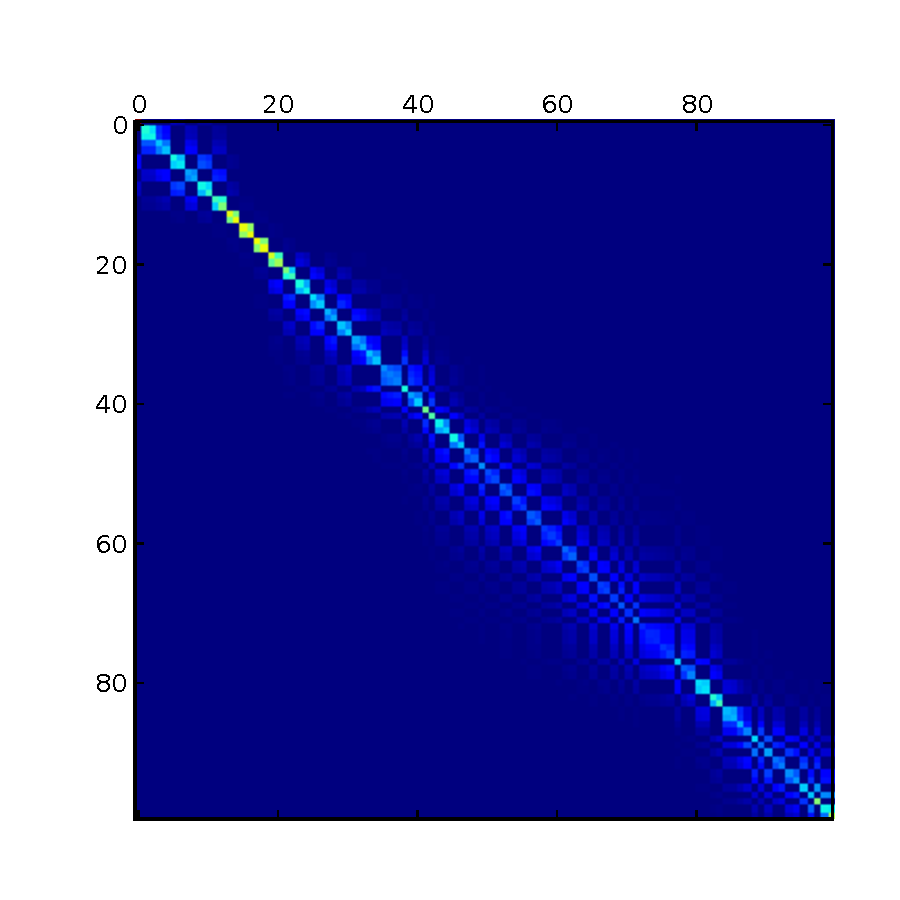
\includegraphics[width=.5\textwidth]{s0_D}
  \caption{An color-coded example dispersion matrix $D$ for the first 100
  trials of subject S0. The used dependence function is a Laplace distribution
  with width $b=2$ for trials of the same class. The green diagonal entries
  around trial 20 indicate independent trials, while the pattern around trial 60
  indicates a closely packed group of trials that are interdependent.}
  \label{fig:ex_D}
\end{figure}

% Feature extraction
\paragraph{Feature extraction}
After preprocessing, the signals were filtered with a 6th-order Butterworth
bandpass filter with a passband of 8--30~Hz, windows of 1~sec centered on the
moment the key-press was registered were extracted, and the Ledoit-Wolf
covariance estimator \cite{ledoit2004wce} was used to estimate the
channel-covariance in the trial window. Finally, a symmetrical whitening
transform $P = \Sigma^{-\frac{1}{2}}$ based on the mean channel covariance
matrix $\Sigma$ was calculated on the training set, and applied to all trials.
The resulting $32\times32$ features were vectorized and used for
classification. This pipeline is conceptually similar to the popular \ac{CSP}
based \cite{koles1991qet, ramoser2000osf} classification of \ac{ERD} related to
movement imagery, but it delegates learning of the spatial filters to the
classifier. 

\paragraph{Performance evaluation}
For \ac{BCI} data it is expected that the \ac{IID} data assumption does not
hold, as there are non-stationary perturbations in the data. This complicates
the evaluation procedure as one cannot simply use cross-validation when the
trials (instances) are inter-dependent. We opted for a simulation
approach, in which we used the first 800 trials for training, used the
performance on the following 400 trials for model selection, and used the
remaining $\approx 800$ trials as the test set. Nevertheless, non-stationary
perturbations could be present in the validation and test set, and could skew
the results, as the performance is measured based on the \ac{IID} assumption.
To improve the robustness of the performance measure, both the validation and
test sets were split into five continuous parts, and the median of the
performance on each part was used.
%
As a measure of performance we chose to use the \ac{ITR} based on \ac{MI}
between the predictions and the true class labels, which is an
information-theoretic measure of the communication speed through an unreliable
communication channel (the \ac{BCI}). The advantage of \ac{ITR} over, for
example, accuracy is that it takes both the quality of the prediction and the
speed of communication into account.

\begin{table}
  \caption{The \protect\ac{ITR} for the \protect\ac{SVM} and \protect\ac{dSVM}
  classifiers. \protect\acp{ITR} below 1 bit/min have been removed for clarity.} 
  \label{tab:dsvm_itr}
  \begin{center}

  \begin{tabular}{c D{.}{.}{3} D{.}{.}{3} D{.}{.}{2}}
    \toprule
    Subject & 
      \multicolumn{1}{c}{\ac{SVM} bits/min} & 
      \multicolumn{1}{c}{\ac{dSVM} bits/min} & 
      \multicolumn{1}{c}{b-param}\\
    \midrule
    S0 & 5.26 & 6.38 & 1.3\\
    S1 & - & - & 0.01\\
    S2 & - & - & 8.9\\
    S3 & - & - & 0.48\\
    S4 & - & 1.02 & 0.11\\
    S5 & 11.9 & 11.2 & 0.11\\
    S6 & - & - & 5.5\\
    S7 & - & - & 38\\
    S8 & - & - & 8.9\\
    S9 & 13.8 & 18.0 & 0.3\\
    S10 & 2.58 & 5.1 & 1.3\\
    S11 & -& - & 2.1\\
    \bottomrule
  \end{tabular}
  \end{center}
\end{table}

\begin{figure}
  \center
  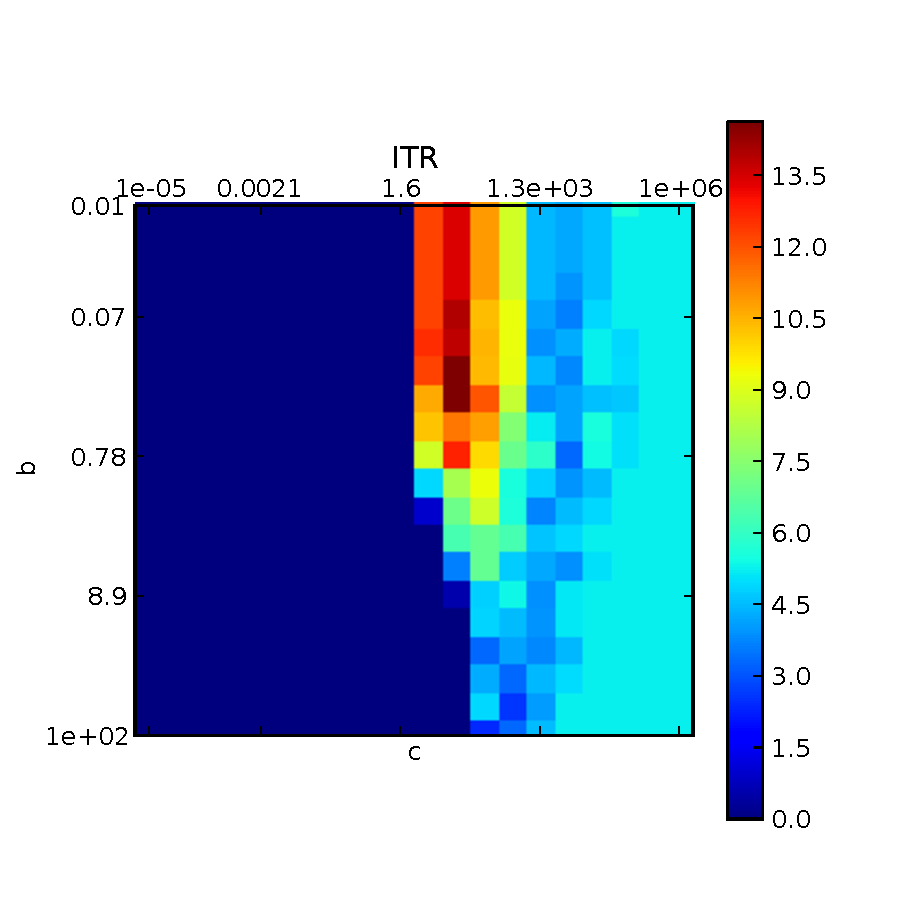
\includegraphics[width=.5\textwidth]{s9_itr_grid}
  \caption{The \protect\ac{ITR} on the test set of S9 for different
  combinations of the cost parameter $c$ and dispersion parameter $b$. The top
  row has such a small $b$ that the \protect\ac{dSVM} degenerates in the
  traditional \protect\ac{SVM}. The optimal spread appears to be $b=0.3$, which
  indicates that modeling the inter-dependency of trials is beneficial for this
  subject.}
  \label{fig:s9_itrgrid}
\end{figure}

\paragraph{Results} 
On the training and validation set, we performed a grid-search with the
soft-margin \acp{SVM} and the \acp{dSVM} with different cost parameters $c$,
and different width parameters $b$ in \eqref{eq:dfunc} for the \ac{dSVM} (see
Figure~\ref{fig:ex_D} for an example of the resulting $D$) with a linear,
inhomogeneous kernel. The offset parameter $\mu$ in \eqref{eq:dfunc} was set to
zero.
%
The performance of the selected \ac{SVM} and \ac{dSVM} classifiers are
presented in Table~\ref{tab:dsvm_itr}. Unfortunately, for a number of subjects
no well-performing classifier could be trained with either classifier. For the
subjects for which a classifier could be trained, the \ac{dSVM} seems to
outperform the standard soft-margin \ac{SVM}, with S5 being the only (minor)
exception. The best subject displays a dramatic improvement in performance,
from 13.8 to 18.0 bits per minute (see Figure~\ref{fig:s9_itrgrid}).


\section{Discussion}
\section{Discussion}
The results indicate that the new \acl{SOB} covariance features provide a
robust alternative to \ac{CSP} features for classification of motor imagery,
and generalize to new, unseen subjects without additional calibration or
training. Apparently, the normalization performed with the \ac{SOB} removes
enough inter-subject variability to generalize to new subjects.
%
However, the dataset used in this research contains rather few trials, hence
the \ac{SD} \ac{CSP} performance might have suffered from insufficient training
data. Nevertheless, recording more trials is not always an option, and the
\ac{SD} performance obtained in our study is similar to scores presented in
\cite{fazli2009sim} where much longer sessions were used. Further, when a
similar \ac{SD} \ac{CSP} pipeline with a broadband spectral filter was applied
to naive (i.e. users that have not used a \ac{BCI} before) users in
\cite{blankertz2008bbc}, the results were barely above chance although
280 trials were available for evaluation. The performance increased
dramatically though when subject-specific \emph{spectral} filters were used. 

The \ac{SOB}'s $\alpha$ parameter seems of some importance for generalization
over subjects. While for \ac{SD} classification a long half-life was preferred,
$\alpha$'s with a short half-life were preferred for \ac{SI} classification.
%
Presumably, slow adaptation is preferred for \ac{SD} classification because it
allows the classifier to model and exploit session-specific variations, such as
for example bad channels and \ac{EEG} artifacts. For \ac{SI} classifications
modeling these variations is generally not helpful as they are not consistent
over subjects. Shorter half-lives reduce these variations, and are thus
preferred for \ac{SI} classification.
 
\begin{sloppypar}
It is noteworthy to mention that the best $\alpha$-value for
\ac{SOB}-covariance features was selected based on the performance on
the test subjects. This might slightly overestimate the true performance. 
%
Usually these hyper-parameters (e.g. the \ac{SVM}'s $c$-parameter) are set
based on performance estimates obtained with cross-validation. The half-life
constant $\alpha$ could be chosen with cross-validation, but since the \ac{SOB}
is a preprocessing method this is often computationally impractical.
%
Since current \ac{BCI} pipelines have several preprocessing hyper-parameters
that are fixed a priori (e.g. the cut-off values in the band-pass filter, or
the $m=6$ spatial filters), we can imagine that a fixed $\alpha$ can be used as
well. Given that even the worst $\alpha$ performs better than the alternatives
in \ac{SI} classification, the performance gain seems fairly robust for a wide
range of $\alpha$-values (Fig.~\ref{fig:csob_acc}). Therefore, we expect that
choosing $\alpha=0.16$ (a half-life of 4 trials) a priori will be adequate in
practice. This value is probably independent of the mental task used.
\end{sloppypar}


\section{Conclusions and future work}
\section{Conclusions and future work}
\begin{sloppypar}
We have presented an \ac{SOB} procedure that reduces inter-subject and
inter-session variability, and demonstrated that \ac{SOB}-covariance features
allow for cross-subject motor imagery classification without a loss of
performance compared to within-subject classification with the popular \ac{CSP}
based \ac{BCI} classifier.
%
The advantage of the \ac{SOB} based covariance features is that they are robust
against inter-session and inter-subject variation, and that standard
classifiers such as the \ac{SVM} can be used without the need of any adaptation
or post-processing of the outputs (e.g. bias-adaptation).
%
Furthermore, the online processing is simplified as it can be implemented as a
stateless, fixed pipeline that does not handle the incoming data differently
during a calibration session.

In addition to the practical advantages of removing the need for the laborious
calibration sessions, changing from \acl{SD} to \acl{SI} \acp{BCI} also
simplifies multi-disciplinary \ac{BCI} research. It allows researchers to work
with validated \ac{BCI} classifiers that are known to work with a certain
probability on the target population, and focusses on the intended brain
regions.
% 
The development of \acl{SI} \acp{BCI} can facilitate new applications for which
collecting enough subject-specific training data before each session is not
feasible, such as for example fatigue detection, screening of neurological
disorders or classification of emotional states.
\end{sloppypar}

The method described uses a single, broad frequency band. For future work, the
features can be extended to include multiple frequency bands as in
\cite{lotte2009cdt, farquhar2009lfs}. Work with naive \ac{BCI} users has shown that subject-specific frequency bands can dramatically improve performance \cite{blankertz2008bbc}.
 
\begin{sloppypar}
Another interesting research direction is to generalize to recordings with
different electrode layouts. As the learned covariance weights were quite
sparse, the correspondence of a few key sensor locations might be enough to
generalize to new sensor configurations. This sparsity in covariance space
seems to suggest that it is more natural to think in covariance (or coherence)
between brain regions, than to think of power in spatially filtered sources.
The second row in Figure~\ref{fig:ud_patt} shows spatial filters with a dipolar
structure on the motor cortices. The combination of these and many more filters
is needed to isolate a specific covariance pair --- that is, the intriguing
dipolar structure is probably residue caused by the decomposition of the weight
matrix.
\end{sloppypar}

Finally, although the method presented works causally, it should be validated in
an online experiment with a user in the loop.

